% LuaLaTeX

\documentclass[a4paper, twoside, 12pt]{article}
\usepackage[latin]{babel}
%\usepackage[landscape, left=3cm, right=1.5cm, top=2cm, bottom=1cm]{geometry} % okraje stranky
%\usepackage[landscape, a4paper, mag=1166, truedimen, left=2cm, right=1.5cm, top=1.6cm, bottom=0.95cm]{geometry} % okraje stranky
\usepackage[landscape, a4paper, mag=1400, truedimen, left=0.5cm, right=0.5cm, top=0.5cm, bottom=0.5cm]{geometry} % okraje stranky

\usepackage{fontspec}
\setmainfont[FeatureFile={junicode.fea}, Ligatures={Common, TeX}, RawFeature=+fixi]{Junicode}
%\setmainfont{Junicode}

% shortcut for Junicode without ligatures (for the Czech texts)
\newfontfamily\nlfont[FeatureFile={junicode.fea}, Ligatures={Common, TeX}, RawFeature=+fixi]{Junicode}

\usepackage{multicol}
\usepackage{color}
\usepackage{lettrine}
\usepackage{fancyhdr}

% usual packages loading:
\usepackage{luatextra}
\usepackage{graphicx} % support the \includegraphics command and options
\usepackage{gregoriotex} % for gregorio score inclusion
\usepackage{gregoriosyms}
\usepackage{wrapfig} % figures wrapped by the text
\usepackage{parcolumns}
\usepackage[contents={},opacity=1,scale=1,color=black]{background}
\usepackage{tikzpagenodes}
\usepackage{calc}
\usepackage{longtable}
\usetikzlibrary{calc}

\setlength{\headheight}{14.5pt}

% Commands used to produce a typical "Conventus" booklet

\newenvironment{titulusOfficii}{\begin{center}}{\end{center}}
\newcommand{\dies}[1]{#1

}
\newcommand{\nomenFesti}[1]{\textbf{\Large #1}

}
\newcommand{\celebratio}[1]{#1

}

\newcommand{\hora}[1]{%
\vspace{0.5cm}{\large \textbf{#1}}

\fancyhead[LE]{\thepage\ / #1}
\fancyhead[RO]{#1 / \thepage}
\addcontentsline{toc}{subsection}{#1}
}

% larger unit than a hora
\newcommand{\divisio}[1]{%
\begin{center}
{\Large \textsc{#1}}
\end{center}
\fancyhead[CO,CE]{#1}
\addcontentsline{toc}{section}{#1}
}

% a part of a hora, larger than pars
\newcommand{\subhora}[1]{
\begin{center}
{\large \textit{#1}}
\end{center}
%\fancyhead[CO,CE]{#1}
\addcontentsline{toc}{subsubsection}{#1}
}

% rubricated inline text
\newcommand{\rubricatum}[1]{\textit{#1}}

% standalone rubric
\newcommand{\rubrica}[1]{\vspace{3mm}\rubricatum{#1}}

\newcommand{\notitia}[1]{\textcolor{red}{#1}}

\newcommand{\scriptura}[1]{\hfill \small\textit{#1}}

\newcommand{\translatioCantus}[1]{\vspace{1mm}%
{\noindent\footnotesize \nlfont{#1}}}

% pruznejsi varianta nasledujiciho - umoznuje nastavit sirku sloupce
% s prekladem
\newcommand{\psalmusEtTranslatioB}[3]{
  \vspace{0.5cm}
  \begin{parcolumns}[colwidths={2=#3}, nofirstindent=true]{2}
    \colchunk{
      \input{#1}
    }

    \colchunk{
      \vspace{-0.5cm}
      {\footnotesize \nlfont
        \input{#2}
      }
    }
  \end{parcolumns}
}

\newcommand{\psalmusEtTranslatio}[2]{
  \psalmusEtTranslatioB{#1}{#2}{8.5cm}
}


\newcommand{\canticumMagnificatEtTranslatio}[1]{
  \psalmusEtTranslatioB{#1}{temporalia/extra-adventum-vespers/magnificat-boh.tex}{12cm}
}
\newcommand{\canticumBenedictusEtTranslatio}[1]{
  \psalmusEtTranslatioB{#1}{temporalia/extra-adventum-laudes/benedictus-boh.tex}{10.5cm}
}

% volne misto nad antifonami, kam si zpevaci dokresli neumy
\newcommand{\hicSuntNeumae}{\vspace{0.5cm}}

% prepinani mista mezi notovymi osnovami: pro neumovane a neneumovane zpevy
\newcommand{\cantusCumNeumis}{
  \setgrefactor{17}
  \global\advance\grespaceabovelines by 5mm%
}
\newcommand{\cantusSineNeumas}{
  \setgrefactor{17}
  \global\advance\grespaceabovelines by -5mm%
}

% znaky k umisteni nad inicialu zpevu
\newcommand{\superInitialam}[1]{\gresetfirstlineaboveinitial{\small {\textbf{#1}}}{\small {\textbf{#1}}}}

% pars officii, i.e. "oratio", ...
\newcommand{\pars}[1]{\textbf{#1}}

\newenvironment{psalmus}{
  \setlength{\parindent}{0pt}
  \setlength{\parskip}{5pt}
}{
  \setlength{\parindent}{10pt}
  \setlength{\parskip}{10pt}
}

%%%% Prejmenovat na latinske:
\newcommand{\nadpisZalmu}[1]{
  \hspace{2cm}\textbf{#1}\vspace{2mm}%
  \nopagebreak%

}

% mode, score, translation
\newcommand{\antiphona}[3]{%
\hicSuntNeumae
\superInitialam{#1}
\includescore{#2}

#3
}
 % Often used macros
%%%% Preklady jednotlivych zpevu (nektere se opakuji, a je dobre mit je
% vsechny na jedne hromade)

\newcommand{\trOratioAnteOfficium}{\translatioCantus{Otevři, Pane, má ústa, abych chválil tvé svaté jméno.
Očisti mé srdce od všech marnivých, zvrácených a~jiných myšlenek, osvěť rozum, rozněť cit,
abych mohl důstojně, soustředěně a~zbožně recitovat a~vysloužil si být
vyslyšen před tváří tvé velebnosti. Skrze Krista…}}

\newcommand{\trOratioPostOfficium}{\translatioCantus{\textit{Následující modlitbu
opatřil pro ty, kdo ji zbožně vyřknou po hodinkách, zesnulý papež Lev X.
odpustky za hříchy vzniklé při konání hodinek z~lidské křehkosti. Říká se
vkleče.}
Svatosvaté a~nerozdílné Trojici, ukřižovanému lidství našeho Pána Ježíše
Krista, přeblažené a~přeslavné plodné neporušenosti vždy Panny Marie
i~souhrnu všech svatých buď ode všeho stvoření věčná chvála, čest a~sláva, nám
pak buď dáno odpuštění všech hříchů, po nekonečné věky věků. Amen.}}

% HOURS ---

\newcommand{\trAntI}{\translatioCantus{Jasné narození slavné Panny Marie,
z pokolení (dosl. ze semene) Abrahámova, vzešlé z kmene Judova, z rodu Davidova.}}
\newcommand{\trAntII}{\translatioCantus{Dnes je Narození svaté Panny 
Marie, jejíž předrahý život osvěcuje všechny církve.}}

\newcommand{\trAntIII}{\translatioCantus{Maria, jež vzešla 
z královského rodu, září; myslí i duchem ji zbožně prosíme, aby 
nám pomáhala svými přímluvami.}}

\newcommand{\trAntIV}{\translatioCantus{Srdcem i duchem pějme Kristu 
k slávě o této svaté slavnosti vznešené Rodičky Boží Marie.}}

\newcommand{\trAntV}{\translatioCantus{Příjemně \notitia{?} 
oslavujme Narození blahoslavené Marie,
aby se ona za nás přimlouvala u Pána Ježíše Krista.}}

\newcommand{\trCapituli}{\translatioCantus{Před věky, na počátku mě stvořil, potrvám věčně. Ve svatém Stanu jsem před ním konala službu.}}

\newcommand{\trRespVesp}{\translatioCantus{Buď zdráva, Maria,
plná milosti: \grestar{} Pán s tebou. \Vbardot{} Požehnaná jsi mezi ženami,
a požehnaný plod života (ve smyslu lůna, břicha) tvého.}}

\newcommand{\trVersus}{\translatioCantus{\Vbardot{} Dnes je Narození svaté Panny Marie. \Rbardot{} Jejíž předrahý život osvěcuje všechny církve.}}

\newcommand{\trAntMagnificatI}{\translatioCantus{Konejme památku
veledůstojného narození slavné Panny Marie,
jíž se dostalo mateřské důstojnosti bez ztráty panenské cudnosti.}}

% Tento preklad je vice nez nejisty a ani alternativy, ktere jsem
% videl, me nepresvedcily...
\newcommand{\trAntBenedictus}{\translatioCantus{Slavnostně slavme 
dnešní narození Marie, vždy Panny a Rodičky Boží: v něm se objevuje
vysokost trůnu (totiž Marie, trůnu Božího Syna), aleluja.}}

\newcommand{\trAntMagnificatII}{\translatioCantus{Tvé narození,
Bohorodičko Panno, vyhlásilo radost celému světu:
z tebe totiž vzešlo Slunce spravedlnosti, Kristus, náš Bůh:
jenž zrušil kletbu a dal nám požehnání: přemohl smrt a dal nám život věčný.}}

\newcommand{\trOrationis}{\translatioCantus{Prosíme tě, Bože, 
uděl svým služebníkům dar nebeské milosti,
aby těm, jimž slehnutím blahoslavené Panny vyvstal počátek spásy, 
slavnost k poctě jejího narození přinesla
rozhojnění pokoje.
Skrze tvého Syna, našeho Pána Ježíše Krista, který s tebou žije a kraluje,
Bůh, v jednotě Ducha svatého po všechny věky věků.}}

\newcommand{\trFideliumAnimae}{\translatioCantus{\Vbardot{} Duše věrných ať pro
milosrdenství Boží odpočívají v~pokoji. \Rbardot{} Amen.}}

% Completorium

\newcommand{\trJubeDomne}{\translatioCantus{Rač, pane, požehnat.}}

\newcommand{\trComplBenedictio}{\translatioCantus{Pokojnou noc a~svatou smrt
nechť nám dopřeje všemohoucí Pán. \Rbardot{} Amen.}}

\newcommand{\trComplLectioBr}{\translatioCantus{Buďte střízliví, bděte.
Váš protivník Ďábel obchází jako lev řvoucí a~hledá, koho by pohltil.
Postavte se proti němu pevní ve víře.  Ale ty, Pane, smiluj se nad námi.
\Rbardot{} Bohu díky.}}

\newcommand{\trComplAntI}{\translatioCantus{Rač se smilovati nade mnou,
Hospodine, a vyslyš mou modlitbu.}}

\newcommand{\trComplCapituli}{\translatioCantus{Jsi přece, Hospodine,
uprostřed nás a~jmenujeme se po tobě.  Neopouštěj nás, Pane, náš Bože.}}

\newcommand{\trRespCompl}{\translatioCantus{Do tvých rukou, Pane, \grestar{}
poroučím svého ducha. \Vbardot{} Ty mne zachráníš, Pane, Bože věrný.}}

\newcommand{\trComplVersus}{\translatioCantus{\Vbardot{} Střez mne jako zřítelnici oka,
aleluja. \Rbardot{} Ve stínu svých křídel uschovej mne, aleluja.}}

\newcommand{\trAntSalvaNos}{\translatioCantus{Ochraňuj nás, Pane, když
bdíme, a~buď s~námi, když spíme, ať bdíme s~Kristem a~odpočíváme v~pokoji.}}

\newcommand{\trComplOrationis}{\translatioCantus{Zavítej, prosíme, Pane, sem
do našeho příbytku a~daleko od něj zažeň všechny úklady nepřítele. Ať tu
bydlí tví svatí andělé a~tvoje požehnání buď nad ním stále. Skrze…}}

\newcommand{\trSalveRegina}{\translatioCantus{Zdrávas Královno, matko
milosrdenství, živote, sladkosti a naděje naše, buď zdráva!
K tobě voláme, vyhnaní synové Evy,
k tobě vzdycháme, lkajíce a plačíce
v tomto slzavém údolí.
A proto, orodovnice naše,
obrať k nám své milosrdné oči
a Ježíše, požehnaný plod života svého,
nám po tomto putování ukaž,
ó milostivá, ó přívětivá,
ó přesladká, Panno Maria!}}

\newcommand{\trOraProNobis}{\translatioCantus{\Vbardot{} 
Oroduj za nás, svatá Boží Rodičko,
\Rbardot{} aby nám Kristus dal účast na svých zaslíbeních.}}

% Matutinum

\newcommand{\trMatInvitatorium}{\translatioCantus{}}

\newcommand{\trMatVeniteA}{\translatioCantus{Pojďte, chvalme s~radostí Pána,
s~jásotem slavme Boha, svou spásu; předstupme před tvář jeho s~díky, písně plesu pějme jemu.}}

\newcommand{\trMatVeniteB}{\translatioCantus{Neboť Bůh veliký jest Hospodin, a~král nade všecky bohy.
Jsouť v~jeho ruce všecky hlubiny země, temena hor jsou majetek jeho.}}

\newcommand{\trMatVeniteC}{\translatioCantus{Jehoť jest moře, neb on je učinil; i~souš
je dílo jeho rukou. Pojďme, klanějme se, padněme, klekněme před Pánem, svým
tvůrcem. Jeť on Pán, náš Bůh, a~my jsme lid, jejž on vodí a~ovce, jež pase.}}

\newcommand{\trMatVeniteD}{\translatioCantus{Kéž byste poslechli dnes hlasu jeho:
,,Nezatvrzujte svých srdcí jak v~Hádce, jak v~Pokušení na poušti, kde vaši otcové pokoušeli mne,
zkoušeli mne, ač vídali skutky mé.``}}

\newcommand{\trMatVeniteE}{\translatioCantus{Čtyřicet roků mrzel jsem se na to pokolení
a~řekl jsem: ,,Lid je to myslí stále bloudící``! Oni však nechtěli znáti mé cesty, takže jsem
přisáhl ve svém hněvu: ,,Nedojdou odpočinku mého!\mbox{}``}}

\newcommand{\trMatAntI}{\translatioCantus{}}

\newcommand{\trMatAntII}{\translatioCantus{}}

\newcommand{\trMatAntIII}{\translatioCantus{}}

\newcommand{\trMatVersusI}{\translatioCantus{}}

\newcommand{\trMatAbsolutioI}{\translatioCantus{Vyslyš Pane Ježíši Kriste
prosby svých služebníků \gredagger{} a~smiluj se nad námi, \grestar{} jenž
s~Otcem a~Duchem…}}

\newcommand{\trMatBenedictioI}{\translatioCantus{Rač, pane, požehnat.
Věčný Otec nám stále žehnej. \Rbardot{} Amen.}}

\newcommand{\trMatLecI}{\translatioCantus{Kéž by mě zulíbal polibky svých úst. 
Tvé milování je nad víno lahodnější;
vybraně voní tvé voňavky;
rozlévající se olej je tvé jméno,
proto tě dívky milují.
Strhni mě za sebou, poběžme!
Král mě uvedl do svých komnat;
budeš nám radostí a jásotem.
Víc než víno oslavíme tvé milování;
věru po právu jsi milován!
Snědá jsem, a přece krásná, jeruzalémské dcery,
jako stany kedarské,
jako šalmské závěsy.
}}

\newcommand{\trMatRespI}{\translatioCantus{}}

\newcommand{\trMatBenedictioII}{\translatioCantus{Rač, pane, požehnat.
Jednorozený Boží Syn nám žehnej \grestar{} a nám pomáhej. \Rbardot{} Amen.}}

\newcommand{\trMatLecII}{\translatioCantus{Nehleďte na mou osmahlou pleť:
to mě slunce ožehlo.
Synové mé matky se na mne rozzlobili,
poslali mě hlídat vinice.
A svou vinici, tu jsem nehlídala!
Pověz mi tedy, ty, jehož miluje mé srdce:
kam zavedeš své stádo pást,
kde ho necháš za poledne odpočívat?
Abych už nebloudila jako tulačka
poblíž stád druhů tvých.
Nevíš-li to, nejrásnější z žen,
jdi po stopách stáda
a kůzlata svá zaveď, ať se pasou
poblíž obydlí pastýřů.
Ke své klisně zapřažené do vozu faraonova
tebe, mé milá, přirovnávám.
Stále krásné jsou tvé líce s náušnicemi
i tvé hrdlo v náhrdelnících.}}

\newcommand{\trMatRespII}{\translatioCantus{}}

\newcommand{\trMatBenedictioIII}{\translatioCantus{Rač, pane, požehnat.
Milost Ducha Svatého ať osvítí nám smysly \grestar{} i srdce. \Rbardot{} Amen.}}

\newcommand{\trMatLecIII}{\translatioCantus{Zhotovíme ti zlaté náušnice
a kuličky ze stříbra.
Když král stoluje,
vydechuje můj nard svou vůni.
Můj milý je polštářek s myrhou,
jenž mi odpočívá mezi ňadry.
Můj milý je hrozen šáchoru
ve vinicích v Engadi.
Jak jsi krásná, milá moje,
jak jsi krásná!
Tvé oči jsou holubice.
Jak jsi krásný, můj milý,
jak líbezný!
Naše lože je samá zeleň.
Trámoví našeho domu je z cedru,
naše ostění z cypřiše.}}

\newcommand{\trMatRespIII}{\translatioCantus{}}

\newcommand{\trMatAntIV}{\translatioCantus{}}

\newcommand{\trMatAntV}{\translatioCantus{}}

\newcommand{\trMatAntVI}{\translatioCantus{}}

\newcommand{\trMatVersusII}{\translatioCantus{}}

\newcommand{\trMatAbsolutioII}{\translatioCantus{
Tvá milost a laskavost nechť nám pomáhá, jenž žiješ a vládneš s Otcem a Svatým Duchem na věky věků.}}

\newcommand{\trMatBenedictioIV}{\translatioCantus{Rač, pane, požehnat.
Bůh Otec všemohoucí, \grestar{} buď k nám milostivý a odpouštějící. \Rbardot{} Amen.}}

\newcommand{\trMatLecIV}{\translatioCantus{}}

\newcommand{\trMatRespIV}{\translatioCantus{}}

\newcommand{\trMatBenedictioV}{\translatioCantus{}}

\newcommand{\trMatLecV}{\translatioCantus{}}

\newcommand{\trMatRespV}{\translatioCantus{}}

\newcommand{\trMatBenedictioVI}{\translatioCantus{Rač, pane, požehnat.
Bůh rozněť v nás oheň své lásky. \Rbardot{} Amen.}}

\newcommand{\trMatLecVI}{\translatioCantus{}}

\newcommand{\trMatRespVI}{\translatioCantus{}}

\newcommand{\trMatAntVII}{\translatioCantus{}}

\newcommand{\trMatAntVIII}{\translatioCantus{}}

\newcommand{\trMatAntIX}{\translatioCantus{}}

\newcommand{\trMatVersusIII}{\translatioCantus{}}

\newcommand{\trMatAbsolutioIII}{\translatioCantus{Z okovů našich hříchů,
\grestar{} vysvoboď nás všemohoucí a milosrdný Pán. \Rbardot{} Amen.}}

\newcommand{\trMatBenedictioVII}{\translatioCantus{Rač, pane, požehnat.
Čtení evangelia nechť je nám \grestar{} spásou a ochranou. \Rbardot{} Amen.}}

\newcommand{\trMatLecVIIa}{\translatioCantus{
  Rodokmen Ježíše Krista, syna Davidova, syna Abrahámova:
  Abrahám zplodil Izáka,
  Izák zplodil Jakuba.}}

\newcommand{\trMatLecVIIb}{\translatioCantus{}}

\newcommand{\trMatRespVII}{\translatioCantus{}}

\newcommand{\trMatBenedictioVIII}{\translatioCantus{Rač, pane, požehnat.
\Rbardot{} Amen.}}

\newcommand{\trMatLecVIII}{\translatioCantus{}}

\newcommand{\trMatRespVIII}{\translatioCantus{}}

\newcommand{\trMatBenedictioIX}{\translatioCantus{Rač, pane, požehnat.
Do společnosti občanů nebes \grestar{} ať nás dovede král andělů.
\Rbardot{} Amen.}}

\newcommand{\trMatLecIX}{\translatioCantus{}}

% from the Czech Liturgia horarum
\newcommand{\trTeDeum}{\begin{translatioMulticol}{3}

Bože, tebe chválíme, 
tebe, Pane, velebíme.

Tebe, věčný Otče, 
oslavuje celá země.

Všichni andělé, 
cherubové i~serafové,

všechny mocné nebeské zástupy 
bez ustání volají:

Svatý, Svatý, Svatý, 
Pán, Bůh zástupů.

Plná jsou nebesa i~země 
tvé vznešené slávy.

Oslavuje tě 
sbor tvých apoštolů,

chválí tě 
velký počet proroků,

vydává o~tobě svědectví 
zástup mučedníků;

a~po celém světě 
vyznává tě tvá církev:

neskonale velebný, 
všemohoucí Otče,

úctyhodný Synu Boží, 
pravý a~jediný,

božský Utěšiteli, 
Duchu svatý.

Kriste, Králi slávy, 
tys od věků Syn Boha Otce;

abys člověka vykoupil, 
stal ses člověkem a~narodil ses z~Panny;

zlomil jsi osten smrti 
a~otevřel věřícím nebe;

sedíš po Otcově pravici 
a~máš účast na jeho slávě.

Věříme, že přijdeš soudit, 

a~proto tě prosíme:
přispěj na pomoc svým služebníkům, 
vždyť jsi je vykoupil svou předrahou krví;

dej, ať se radují s~tvými svatými 
ve věčné slávě.

Zachraň, Pane, svůj lid, žehnej svému dědictví, 
veď ho a~stále pozvedej.

Každý den tě budeme velebit 
a~chválit tvé jméno po všechny věky.

Pomáhej nám i~dnes, 
ať se nedostaneme do područí hříchu.

Smiluj se nad námi, Pane, 
smiluj se nad námi.

Ať spočine na nás tvé milosrdenství, 
jak doufáme v~tebe.

Pane, k~tobě se utíkáme, 
ať nejsme zahanbeni na věky. 
\end{translatioMulticol}}

\newcommand{\trMatEvangelium}{\translatioCantus{
  Rodokmen Ježíše Krista, syna Davidova, syna Abrahámova:
  Abrahám zplodil Izáka,
  Izák zplodil Jakuba,
  Jakub zplodil Judu a jeho bratry,
  Juda zplodil Farese a Zaru z Tamary,
  Fares zplodil Esroma,
  Esrom zplodil Arama,
  Aram zplodil Aminadaba,
  Aminadab zplodil Naasona,
  Naason zplodil Salmona,
  Salmon zplodil Boaze z Rahaby,
  Boaz zplodil Jobeda z Rut,
  Jobed zplodil Jessea,
  Jesse zplodil krále Davida.
  David zplodil Šalomouna z Uriášovy ženy,
  Šalomoun zplodil Roboama,
  Roboam zplodil Abiu,
  Abia zplodil Asu,
  Asa zplodil Josafata,
  Josafat zplodil Jorama,
  Joram zplodil Oziáše,
  Oziáš zplodil Joatama,
  Joatam zplodil Achaze,
  Achaz zplodil Ezechiáše,
  Ezechiáš zplodil Manasesa,
  Manases zplodil Amona,
  Amon zplodil Josiáše,
  Josiáš zplodil Jechoniáše a jeho bratry;
  tehdy došlo k odvlečení do Babylonu.
  Po odvlečení do Babylonu:
  Jechoniáš zplodil Salatiela,
  Salatiel zplodil Zorobabela,
  Zorobabel zplodil Abiuda,
  Abiud zplodil Eljakima,
  Eljakim zplodil Azora,
  Ator zplodil Sadoka,
  Sadok zplodil Achima,
  Achim zplodil Eliuda,
  Eliud zplodil Eleazara,
  Eleatar zplodil Matana,
  Matan zplodil Jakuba,
  Jakub zplodil Josefa, manžela Marie,
  z níž se narodil Ježíš, který se nazývá Kristus.}}

\newcommand{\trTeDecetLaus}{\translatioCantus{Tobě chvála, Tobě zpěvy, Tobě
sláva, Bohu Otci i~Synu i~Svatému Duchu, na věky věků. \Rbardot{} Amen.}}

% MASS ---

\newcommand{\trIntroitus}{\translatioCantus{Radujme se všichni
v Pánu, slavíce svátek ke cti Panny Marie: z něj se radují andělé
a spoluchválí Božího Syna. \textit{\color{red}Žl.} Má ústa vydala dobré slovo,
přednáším svá díla králi.}}

\newcommand{\trGraduale}{\translatioCantus{Požehnaná a ctihodná jsi,
Panno Maria: nedotčená (co do panenství) jsi byla shledána matkou
Spasitele. \Vbardot{} Panno Boží Rodičko, ten, jehož nepojme ani celý svět,
se uzavřel do tvých útrob, když se stal člověkem.}}

\newcommand{\trAlleluia}{\translatioCantus{Aleluja. \Vbardot{} Skvělá slavnost
slavné Panny Marie, z pokolení (dosl. ze semene) Abrahámova, vzešlé z kmene 
Judova, z rodu Davidova.}}

\newcommand{\trOffertorium}{\translatioCantus{Blažená jsi, Panno Maria,
tys nosila Stvořitele všeho; porodila jsi toho, který tě utvořil,
a na věky zůstáváš Pannou.}}

\newcommand{\trCommunio}{\translatioCantus{Budou mě blahoslavit
všechna pokolení, protože mi učinil veliké věci ten, který je mocný.}}

% LITTLE HOURS ---

\newcommand{\trVersusTertia}{\translatioCantus{\Vbardot{} \Rbardot{}}}

\newcommand{\trCapituliEtSic}{\translatioCantus{
Tak jsem se usadila na Sionu a v milovaném městě jsem nalezla odpočinek,
v Jeruzalémě vykonávám svou moc.
Zakořenila jsem u lidu plného slývy, na panství Páně, v jeho dědictví.}}

\newcommand{\trVersusSexta}{\translatioCantus{\Vbardot{} \Rbardot{}}}

\newcommand{\trCapituliInPlateis}{\translatioCantus{
Na planině jako skořicovník a akant jsem vydávala vůni, jako vybraná myrha
jsem voněla.}}

\newcommand{\trVersusNona}{\translatioCantus{\Vbardot{} \Rbardot{}}}
 % Czech translations of the proper texts

\newcommand{\annusEditionis}{2022}

%%%% Vicekrat opakovane kousky

\newcommand{\anteOrationem}{
  \rubrica{Ante Orationem, cantatur a Superiore:}

  \pars{Supplicatio Litaniæ.}

  \cuminitiali{}{temporalia/supplicatiolitaniae.gtex}

  \pars{Oratio Dominica.}

  \cuminitiali{}{temporalia/oratiodominica.gtex}

  \rubrica{Deinde dicitur ab Hebdomadario:}

  \cuminitiali{}{temporalia/dominusvobiscum-solemnis.gtex}

  \rubrica{In choro monialium loco Dominus vobiscum dicitur:}

  \sineinitiali{temporalia/domineexaudi.gtex}
}

\newcommand{\capitulumLaudes}{\pars{Capitulum.} \scriptura{Rom. 11, 33}

\grechangedim{interwordspacetext}{0.12 cm plus 0.15 cm minus 0.05 cm}{scalable}%
\cuminitiali{}{temporalia/capitulum-OAltitudo.gtex}
\grechangedim{interwordspacetext}{0.22 cm plus 0.15 cm minus 0.05 cm}{scalable}}

\setlength{\columnsep}{30pt} % prostor mezi sloupci

%%%%%%%%%%%%%%%%%%%%%%%%%%%%%%%%%%%%%%%%%%%%%%%%%%%%%%%%%%%%%%%%%%%%%%%%%%%%%%%%%%%%%%%%%%%%%%%%%%%%%%%%%%%%%
\begin{document}

% Here we set the space around the initial.
% Please report to http://home.gna.org/gregorio/gregoriotex/details for more details and options
\grechangedim{afterinitialshift}{2.2mm}{scalable}
\grechangedim{beforeinitialshift}{2.2mm}{scalable}
\grechangedim{interwordspacetext}{0.22 cm plus 0.15 cm minus 0.05 cm}{scalable}%
\grechangedim{annotationraise}{-0.2cm}{scalable}

% Here we set the initial font. Change 38 if you want a bigger initial.
% Emit the initials in red.
\grechangestyle{initial}{\color{red}\fontsize{38}{38}\selectfont}

\pagestyle{empty}

\newcommand{\vesperas}{
\pars{Psalmus 2.} \scriptura{\textbf{H101}}

\vspace{-0.4cm}

\antiphona{II D}{temporalia/ant-lausetperennisgloria.gtex}

\scriptura{Psalmus 110.}

\initiumpsalmi{temporalia/ps110-initium-ii-D-auto.gtex}

\input{temporalia/ps110.tex} \Abardot{}

\vfill
\pagebreak

\pars{Psalmus 3.} \scriptura{\textbf{H101}}

\vspace{-0.4cm}

\antiphona{III e}{temporalia/ant-glorialaudisresonetinore.gtex}

\scriptura{Psalmus 111.}

\initiumpsalmi{temporalia/ps111-initium-iii-e-auto.gtex}

\input{temporalia/ps111.tex} \Abardot{}

\vfill
\pagebreak

\pars{Psalmus 4.} \scriptura{1 Co. 8, 6; \textbf{H101}}

\vspace{-0.4cm}

\antiphona{V a}{temporalia/ant-exquoomnia.gtex}

\scriptura{Psalmus 112.}

\initiumpsalmi{temporalia/ps112-initium-v-a-auto.gtex}

\input{temporalia/ps112.tex} \Abardot{}

%\vfill

%\vspace{-6mm}

%\antiphona{}{temporalia/ant-videntibusillis.gtex} % repeat the antiphon - new page

\vfill
\pagebreak
}

%%%% Titulni stranka
\begin{titulusOfficii}
\nomenFesti{Dominica Sanctissimæ Trinitatis.}
\celebratio{Duplex 1. classis.}
\end{titulusOfficii}

% graphic
%\vspace{1.5cm}
%\begin{center}
%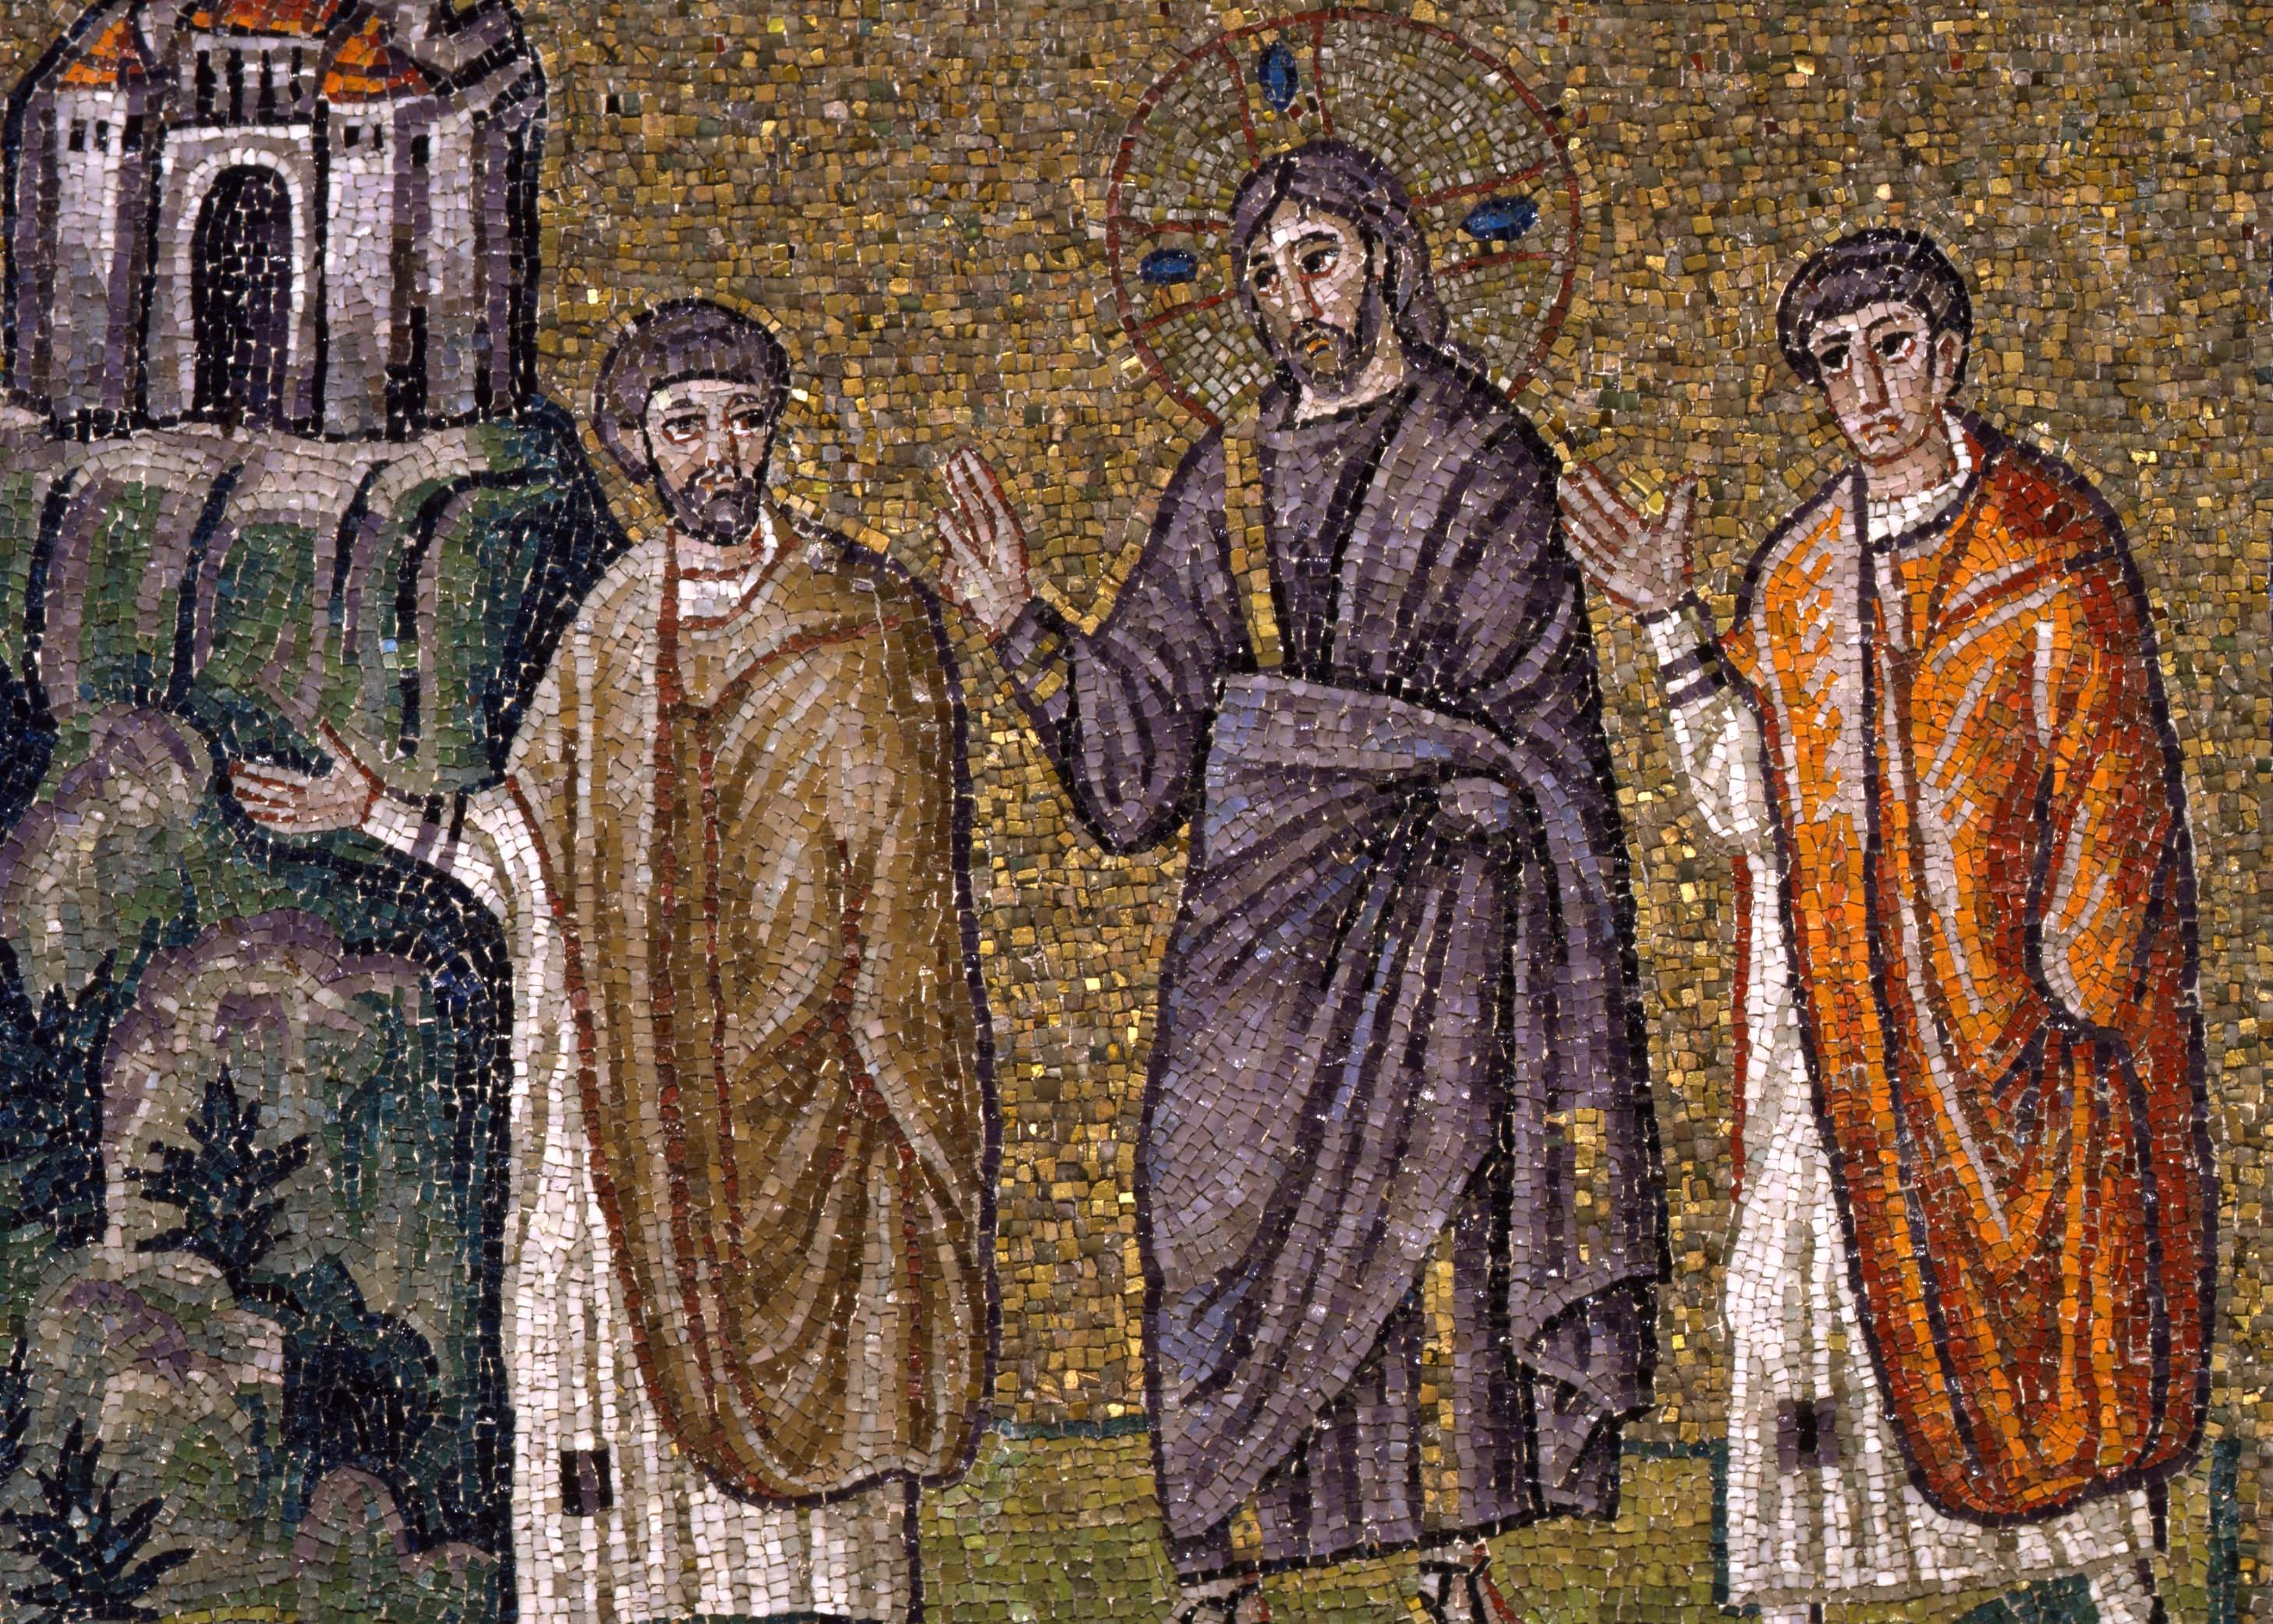
\includegraphics[width=8cm]{emmaus.jpg}
%\end{center}

\vfill

\begin{center}
%Ad usum et secundum consuetudines chori \guillemotright{}Conventus Choralis\guillemotleft.

%Editio Sancti Wolfgangi \annusEditionis
\end{center}

\pagebreak

\renewcommand{\headrulewidth}{0pt} % no horiz. rule at the header
\fancyhf{}
\pagestyle{fancy}

\cantusSineNeumas

\pars{Oratio ante divinum Officium.}

\lettrine{{\color{red}A}}{peri,} Dómine, os meum ad benedicéndum nomen sanctum tuum:
munda quoque cor meum ab ómnibus vanis, pervérsis, et aliénis
cogitatiónibus:
intelléctum illúmina, afféctum inflámma,
ut digne, atténte ac devóte hoc Offícium recitáre váleam,
et exaudíri mérear ante conspéctum Divínæ Maiestátis tuæ.
Per Christum, Dóminum nostrum.
\Rbardot{} Amen.

Dómine, in unióne illíus divínæ intentiónis,
qua ipse in terris laudes Deo persolvísti,
has tibi Horas \rubricatum{(vel \textnormal{hanc tibi Horam})} persólvo.

\vfill

\pars{Oratio post divinum Officium.}

\rubrica{
  Orationem sequentem devote post Officium recitantibus
  Leo Papa X. defectus, et culpas in eo persolvendo ex humana
  fragilitate contractas, indulsit, et dicitur flexis genibus.
}

\lettrine{{\color{red}S}}{acrosánctæ} et indivíduæ Trinitáti,
crucifíxi Dómini nostri Iesu Christi humanitáti,
beatíssimæ et gloriosíssimæ sempérque Vírginis Maríæ
fecúndæ integritáti, 
et ómnium Sanctórum universitáti
sit sempitérna laus, honor, virtus et glória
ab omni creatúra,
nobísque remíssio ómnium peccatórum,
per infiníta sǽcula sæculórum.
\Rbardot{} Amen.

\noindent \Vbardot{} Beáta víscera Maríæ Virginis, quæ portavérunt
ætérni Patris Fílium.\\
\Rbardot{} Et beáta úbera, quæ lactavérunt Christum Dominum.

\rubrica{Et dicitur secreto \textnormal{Pater noster.} et \textnormal{Ave María.}}

\vfill

\hora{Ad I. Vesperas.} %%%%%%%%%%%%%%%%%%%%%%%%%%%%%%%%%%%%%%%%%%%%%%%%%%%%%

\vspace{0.5cm}
\grechangedim{interwordspacetext}{0.18 cm plus 0.15 cm minus 0.05 cm}{scalable}%
\cuminitiali{}{temporalia/deusinadiutorium-solemnis.gtex}
\grechangedim{interwordspacetext}{0.22 cm plus 0.15 cm minus 0.05 cm}{scalable}%

\vfill
\pagebreak

\pars{Psalmus 1.} \scriptura{\textbf{H101}}

\vspace{-0.4cm}

\antiphona{I f}{temporalia/ant-gloriatibitrinitas.gtex}

\scriptura{Psalmus 109.}

\initiumpsalmi{temporalia/ps109-initium-i-f-auto.gtex}

\input{temporalia/ps109.tex} \Abardot{}

\vspace{-1cm}

\vfill
\pagebreak

\vesperas

\capitulumLaudes

\vfill

\iffalse
\pars{Responsorium breve.} \scriptura{Cf. Dan. 3, 57}

\cuminitiali{VI}{temporalia/resp-benedicamuspatrem.gtex}
\else
\pars{Responsorium.} \scriptura{\textbf{H103}}

\cuminitiali{VI}{temporalia/resp-honorvirtus-CROCHU-cumdox.gtex}
\fi

\vfill
\pagebreak

\pars{Hymnus}

\cuminitiali{VIII}{temporalia/hym-OLuxBeata.gtex}
\vspace{-3mm}
%\input{hym-OLuxBeata-bohtext.tex}

\vfill
%\pagebreak

\pars{Versus.} \scriptura{Dan. 3, 56}

% Versus. %%%
\sineinitiali{temporalia/versus-benedictuses.gtex}

\vfill
\pagebreak

\pars{Canticum B. Mariæ V.} \scriptura{\textbf{H102}}

\vspace{-6mm}

{
\grechangedim{interwordspacetext}{0.18 cm plus 0.15 cm minus 0.05 cm}{scalable}%
\antiphona{I d\textsuperscript{3}}{temporalia/ant-gratiastibideus.gtex}
\grechangedim{interwordspacetext}{0.22 cm plus 0.15 cm minus 0.05 cm}{scalable}%
}

\vspace{-3mm}

\scriptura{Lc. 1, 46-55}

\vspace{-2mm}

\cantusSineNeumas
\initiumpsalmi{temporalia/magnificat-initium-isoll-d3.gtex}

\vspace{-1.5mm}

\input{temporalia/magnificat-I.tex} \Abardot{}

\vspace{-1cm}

\vfill
\pagebreak

\anteOrationem

\pagebreak

% Oratio. %%%
\cuminitiali{}{temporalia/oratio.gtex}

\vspace{-1mm}

\vfill

\rubrica{Hebdomadarius dicit iterum Dominus vobiscum, vel cantor dicit:}

\vspace{2mm}

\sineinitiali{temporalia/domineexaudi.gtex}

\rubrica{Postea cantatur a cantore:}

\vspace{2mm}

\cuminitiali{II}{temporalia/benedicamus-solemnism-1vesp.gtex}

\vspace{1mm}

\vfill
\pagebreak

\hora{Ad Matutinum.} %%%%%%%%%%%%%%%%%%%%%%%%%%%%%%%%%%%%%%%%%%%%%%%%%%%%%

\vspace{2mm}

\cuminitiali{}{temporalia/dominelabiamea.gtex}

\vspace{2mm}

\pars{Invitatorium.} \scriptura{Cantor; Psalmus 94; \textbf{H101}}

\vspace{-6mm}

\antiphona{IV}{temporalia/inv-deumverumunum.gtex}

\vfill
\pagebreak

\pars{Hymnus.}

\vspace{-5mm}

\antiphona{IV}{temporalia/hym-AdestoSanctaTrinitas.gtex}

\vfill
\pagebreak

\subhora{In I. Nocturno}

\pars{Psalmus 1.} \scriptura{Cantor; \textbf{H102}}

%\vspace{-5mm}

\antiphona{I d}{temporalia/ant-adestounusdeusomnipotenspater.gtex}

%\vspace{-5mm}

\scriptura{Ps. 8}

%\vspace{-2mm}

\initiumpsalmi{temporalia/ps8-initium-i-d3.gtex}

\input{temporalia/ps8.tex} \Abardot{}

\vfill
\pagebreak

\pars{Psalmus 2.} \scriptura{Cantor; \textbf{H102}}

%\vspace{-5mm}

\antiphona{II D}{temporalia/ant-teunuminsubstantiatrinum.gtex}

%\vspace{-5mm}

\scriptura{Ps. 18}

\initiumpsalmi{temporalia/ps18-initium-ii-D-auto.gtex}

\input{temporalia/ps18.tex}

\vfill

\antiphona{}{temporalia/ant-teunuminsubstantiatrinum.gtex}

\vfill
\pagebreak

\pars{Psalmus 3.} \scriptura{Cantor; \textbf{H102}}

%\vspace{-5mm}

\antiphona{III a}{temporalia/ant-tesemperidemessevivere.gtex}

%\vspace{-5mm}

\scriptura{Ps. 23}

\initiumpsalmi{temporalia/ps23-initium-iii-a.gtex}

\input{temporalia/ps23.tex} \Abardot{}

\vfill
\pagebreak

\pars{Versus.} \scriptura{Cf. Dan. 3, 57}

% Versus. %%%
\sineinitiali{temporalia/versus-benedicamuspatrem.gtex}

\vspace{5mm}

\sineinitiali{temporalia/oratiodominica-mat.gtex}

\vspace{5mm}

\pars{Absolutio.}

\cuminitiali{}{temporalia/absolutio-exaudi.gtex}

\vfill
\pagebreak

\cuminitiali{}{temporalia/benedictio-solemn-benedictione.gtex}

\vspace{7mm}

\pars{Lectio I.} \scriptura{1 Cor. 2, 1-5}

\noindent De Epístola prima beáti Pauli apóstoli ad Corínthios.

\noindent Ego, cum veníssem ad vos, fratres, veni non per sublimitátem sermónis aut sapiéntiæ annúntians vobis mystérium Dei. Non enim iudicávi scire me áliquid inter vos nisi Iesum Christum et hunc crucifíxum. Et ego in infirmitáte et timóre et tremóre multo fui apud vos, et sermo meus et prædicátio mea non in persuasibílibus sapiéntiæ verbis, sed in ostensióne Spíritus et virtútis, ut fides vestra non sit in sapiéntia hóminum sed in virtúte Dei.

\noindent \Vbardot{} Tu autem, Dómine, miserére nobis.
\noindent \Rbardot{} Deo grátias.

\vfill
\pagebreak

\pars{Responsorium 1.} \scriptura{\Rbardot{} Ps. 66, 7.8 \Vbardot{} Ps. 66, 2; \textbf{H102}}

\vspace{-5mm}

\responsorium{I}{temporalia/resp-benedicatnosdeus-sinedox.gtex}{}

\vfill
\pagebreak

\cuminitiali{}{temporalia/benedictio-solemn-unigenitus.gtex}

\vspace{7mm}

\pars{Lectio II.} \scriptura{1 Cor. 2, 6-9}

\noindent Sapiéntiam autem lóquimur inter perféctos, sapiéntiam vero non huius sǽculi neque príncipum huius sǽculi, qui destruúntur, sed lóquimur Dei sapiéntiam in mystério, quæ abscóndita est, quam prædestinávit Deus ante sǽcula in glóriam nostram, quam nemo príncipum huius sǽculi cognóvit; si enim cognovíssent, numquam Dóminum glóriæ crucifixíssent. Sed sicut scriptum est: «Quod óculus non vidit, nec auris audívit, nec in cor hóminis ascéndit, quæ præparávit Deus his, qui díligunt illum».

\noindent \Vbardot{} Tu autem, Dómine, miserére nobis.
\noindent \Rbardot{} Deo grátias.

\vfill
\pagebreak

\pars{Responsorium 2.} \scriptura{\Rbardot{} Ps. 71, 18.19 \Vbardot{} ibidem; \textbf{H102}}

\vspace{-5mm}

\responsorium{II}{temporalia/resp-benedictusdominusdeus-sinedox.gtex}{}

\vfill
\pagebreak

\cuminitiali{}{temporalia/benedictio-solemn-spiritus.gtex}

\vspace{7mm}

\pars{Lectio III.} \scriptura{1 Cor. 2, 10-16}

\noindent Nobis autem revelávit Deus per Spíritum; Spíritus enim ómnia scrutátur, étiam profúnda Dei. Quis enim scit hóminum, quæ sint hóminis, nisi spíritus hóminis, qui in ipso est? Ita et, quæ Dei sunt, nemo cognóvit nisi Spíritus Dei. Nos autem non spíritum mundi accépimus, sed Spíritum, qui ex Deo est, ut sciámus, quæ a Deo donáta sunt nobis; quæ et lóquimur non in doctis humánæ sapiéntiæ, sed in doctis Spíritus verbis, spiritálibus spiritália comparántes. Animális autem homo non pércipit, quæ sunt Spíritus Dei, stultítia enim sunt illi, et non potest intellégere, quia spiritáliter examinántur; spiritális autem iúdicat ómnia, et ipse a némine iudicátur. Quis enim cognóvit sensum Dómini, qui ínstruat eum? Nos autem sensum Christi habémus.

\noindent \Vbardot{} Tu autem, Dómine, miserére nobis.
\noindent \Rbardot{} Deo grátias.

\vfill
\pagebreak

\pars{Responsorium 3.} \scriptura{\Rbardot{} Ps. 76, 14-16 \Vbardot{} ibidem; \textbf{H102}}

\vspace{-5mm}

\responsorium{III}{temporalia/resp-quisdeusmagnus-cumdox.gtex}{}

\vfill
\pagebreak

\subhora{In II. Nocturno}

\pars{Psalmus 4.} \scriptura{Cantor; \textbf{H102}}

\vspace{-5mm}

\antiphona{IV E}{temporalia/ant-teinvocamusteadoramus.gtex}

\vspace{-2mm}

\scriptura{Ps. 46}

\vspace{-1mm}

\initiumpsalmi{temporalia/ps46-initium-iv-E-auto.gtex}

\input{temporalia/ps46.tex} \Abardot{}

\vfill
\pagebreak

\pars{Psalmus 5.} \scriptura{Cantor; \textbf{H103}}

\vspace{-4mm}

\antiphona{V a}{temporalia/ant-spesnostrasalus.gtex}

%\vspace{-3mm}

\scriptura{Ps. 47}

%\vspace{-2mm}

\initiumpsalmi{temporalia/ps47-initium-v-A.gtex}

\vspace{-1.5mm}

\input{temporalia/ps47.tex} \Abardot{}

\vspace{-1cm}

\vfill
\pagebreak

\pars{Psalmus 6.} \scriptura{Cantor; \textbf{H103}}

%\vspace{-5mm}

\antiphona{VI F}{temporalia/ant-liberanossalvanosiustifica.gtex}

%\vspace{-5mm}

\scriptura{Ps. 71}

\initiumpsalmi{temporalia/ps71-initium-vi-F-auto.gtex}

\input{temporalia/ps71.tex}

\vfill

\antiphona{}{temporalia/ant-liberanossalvanos.gtex}

\vfill
\pagebreak

\pars{Versus.} \scriptura{Dan. 3, 56}

\sineinitiali{temporalia/versus-benedictuses-communis.gtex}

\vspace{5mm}

\sineinitiali{temporalia/oratiodominica-mat.gtex}

\vspace{5mm}

\pars{Absolutio.}

\cuminitiali{}{temporalia/absolutio-ipsius.gtex}

\vfill
\pagebreak

\cuminitiali{}{temporalia/benedictio-solemn-deus.gtex}

\vspace{7mm}

\pars{Lectio IV.} \scriptura{Ep. 1 ad Serapionem, 28-30: PG 26, 594-595. 599}

\noindent Ex Epístolis sancti Athanásii epíscopi.

\noindent Haud abs re fúerit véterem traditiónem, doctrinámque ac fidem cathólicæ Ecclésiæ investigáre, quam scílicet Dóminus trádidit, Apóstoli prædicavére et patres servavére. In ea enim Ecclésia fundáta est, a qua si quis excíderit, is nec esse nec ámplius dici christiánus ulla ratióne póterit.

\noindent Itaque Trínitas sancta et perfécta est, quæ in Patre et Fílio et Spíritu Sancto agnóscitur, nihílque aliénum vel extrínsecus admíxtum habet, neque ex creatóre et re creáta constat, sed tota creándi et efficiéndi vi prǽdita est; sibi quoque símilis et indivídua est natúra, unáque eius est efficácia et áctio. Nam Pater per Verbum in Spíritu Sancto ómnia facit, eóque modo Sanctæ Trinitátis únitas servátur. Ita unus Deus in Ecclésia prædicátur, qui est super ómnia et per ómnia et in ómnibus. Super ómnia quidem ut Pater, ut princípium et fons; per ómnia vero, nempe per Verbum; in ómnibus dénique, in Spíritu Sancto.

\noindent \Vbardot{} Tu autem, Dómine, miserére nobis.
\noindent \Rbardot{} Deo grátias.

\vfill
\pagebreak

\pars{Responsorium 4.} \scriptura{\Rbardot{} Ps. 146, 5 \Vbardot{} ibidem; \textbf{H103}}

\vspace{-5mm}

\responsorium{IV}{temporalia/resp-magnusdominus-sinedox.gtex}{}

\vfill
\pagebreak

\cuminitiali{}{temporalia/benedictio-solemn-christus.gtex}

\vspace{7mm}

\pars{Lectio V.}

\noindent Beátus Paulus, cum de spiritálibus rebus ad Corínthios scribit, ómnia ad unum Deum Patrem tamquam ad caput hoc pacto redúcit: Divisiónes vero gratiárum sunt, idem autem Spíritus; et divisiónes ministratiónum sunt, idem autem Dóminus; et divisiónes operatiónum sunt, idem vero Deus, qui operátur ómnia in ómnibus.

\noindent Quæ enim Spíritus síngulis distríbuit, ea a Patre per Verbum dantur. Nam ómnia quæ Patris sunt, item Fílii: unde ea quæ a Fílio in Spíritu dantur, vera sunt Patris múnera. Simíliter cum Spíritus in nobis est, Verbum, a quo illum accípimus, in nobis étiam est, et in Verbo est quoque Pater, atque ita fit istud: Veniémus ego et Pater, et mansiónem apud eum faciémus. Ubi enim lux est, illic et splendor quoque est; ubi item splendor est, ibi simíliter et eius efficiéntia et spléndida est grátia.

\noindent \Vbardot{} Tu autem, Dómine, miserére nobis.
\noindent \Rbardot{} Deo grátias.

\vfill
\pagebreak

\pars{Responsorium 5.} \scriptura{\Vbardot{} Ex Hymno Plasmator hominis; \textbf{H103}}

\vspace{-5mm}

\responsorium{V}{temporalia/resp-gloriapatri-CROCHU.gtex}{}

\vfill
\pagebreak

\cuminitiali{}{temporalia/benedictio-solemn-ignem.gtex}

\vspace{7mm}

\pars{Lectio VI.}

\noindent Quod idem Paulus in secúnda Epístola ad Corínthios his verbis docet: Grátia Dómini nostri Iesu Christi, et cáritas Dei, et communicátio Sancti Spíritus sit cum ómnibus vobis. Grátia enim et donum quod in Trinitáte datur, datur a Patre per Fílium in Spíritu Sancto. Nam quemádmodum ex Patre per Fílium datur grátia, ita in nobis fíeri non potest doni communicátio nisi in Spíritu Sancto. Huius síquidem partícipes effécti, Patris caritátem, Fílii grátiam et ipsíus Spíritus communicatiónem habémus.

\noindent \Vbardot{} Tu autem, Dómine, miserére nobis.
\noindent \Rbardot{} Deo grátias.

\vfill
\pagebreak

\pars{Responsorium 6.} \scriptura{\textbf{H103}}

\vspace{-5mm}

\responsorium{VI}{temporalia/resp-honorvirtus-CROCHU-cumdox.gtex}

\vfill
\pagebreak

\subhora{In III. Nocturno}

\pars{Psalmus 7.} \scriptura{2 Cor. 13, 13; \textbf{H102}}

\vspace{-6mm}

\antiphona{VII a}{temporalia/ant-caritaspaterestgratia.gtex}

\vspace{-1mm}

\scriptura{Ps. 86}

\vspace{-2mm}

\initiumpsalmi{temporalia/ps86-initium-vii-a-auto.gtex}

\input{temporalia/ps86.tex} \Abardot{}

\vfill
\pagebreak

\pars{Psalmus 8.} \scriptura{Boetius de Trinitate; \textbf{H103}}

\vspace{-5mm}

\antiphona{VIII G\textsuperscript{2}}{temporalia/ant-veraxestpaterveritas.gtex}

\vspace{-4mm}

\scriptura{Ps. 95}

\initiumpsalmi{temporalia/ps95-initium-viii-G5.gtex}

\input{temporalia/ps95viiiG.tex} \Abardot{}

\vfill
\pagebreak

\pars{Psalmus 9.} \scriptura{Cantor; \textbf{H103}}

\vspace{-5mm}

\antiphona{VIII G\textsuperscript{5}}{temporalia/ant-unaigiturpaterlogos.gtex}

\vspace{-4mm}

\scriptura{Ps. 97}

\initiumpsalmi{temporalia/ps97-initium-viii-G5.gtex}

\input{temporalia/ps97viiiG.tex} \Abardot{}

\vfill
\pagebreak

\pars{Versus.} \scriptura{Ps. 32, 6}

\sineinitiali{temporalia/versus-verbodomini.gtex}

\vspace{5mm}

\sineinitiali{temporalia/oratiodominica-mat.gtex}

\vspace{5mm}

\pars{Absolutio.}

\cuminitiali{}{temporalia/absolutio-avinculis.gtex}

\vfill
\pagebreak

\cuminitiali{}{temporalia/benedictio-solemn-evangelica.gtex}

\vspace{7mm}

\pars{Lectio VII.} \scriptura{Io. 16, 12-15}

\noindent \noindent Léctio sancti Evangélii secúndum Ioánnem.

\noindent In illo témpore: Dixit lesus discípulis suis: "Adhuc multa hábeo vobis dícere, sed non potéstis portáre modo." Et réliqua.

\vspace{5mm}

\scriptura{Tract. 99,4 : CCL 36,584-585}

\noindent Ex Tractátibus sancti Augustíni epíscopi in Ioánnem.

\noindent Non miréris quod ineffábilis Dei sciéntia, qua novit ómnia, per vários humánæ locutiónis modos, ómnium corporálium sénsuum nomínibus nuncupátur, cum et ipsa mens nostra, hoc est homo intérior, cui unifórmiter sciénti per hos quinque véluti núntios córporis divérsa nuntiántur, quando immutábilem veritátem intéllegit, éligit, díligit, et lumen videt de quo dícitur: \emph{Erat lumen verum,} et verbum audit de quo dícitur: \emph{In princípio erat Verbum,} et odórem capit de quo dícitur: \emph{Post odórem unguentórum tuórum currémus,} et fontem bibit, de quo dícitur: \emph{Apud te est fons vitæ,} et tactu frúitur de quo dícitur: \emph{Mihi autem adhærére Deo bonum est;} nec áliud atque áliud, sed una intellegéntia tot sénsuum nomínibus nuncupátur.

\noindent \Vbardot{} Tu autem, Dómine, miserére nobis.
\noindent \Rbardot{} Deo grátias.

\vfill
\pagebreak

\pars{Responsorium 7.} \scriptura{\textbf{H104}}

\vspace{-5mm}

\responsorium{VII}{temporalia/resp-summaetrinitati-CROCHU.gtex}{}

\vfill
\pagebreak

\cuminitiali{}{temporalia/benedictio-solemn-divinum.gtex}

\vspace{7mm}

\pars{Lectio VIII.}

\noindent Cum ergo de Spíritu Sancto dícitur: \emph{Non enim loquétur a semetípso, sed quxcumque áudiet loquétur,} multo magis ibi simplex natúra, ubi veríssime simplex est, vel intellegénda est vel credénda, quæ longe altéque natúram nostræ mentis excédit. Mutábilis quippe est mens nostra, quæ perdpit discéndo quod nesciébat, et amíttit dediscéndo quod sciébat, et veri similitúdine fállitur, ut pro vero ápprobet falsum, et obscuritáte sua quasi quibúsdam ténebris impedítur, ne pervéniat ad verum.

\noindent Et ídeo non est ista substántia mens nostra veríssime simplex, cui non hoc est esse quod nosse; potest enim esse nec nosse. At illa divína non potest, quia id quod habet est. Ac per hoc non sic habet sciéntiam, ut áliud illi sit sciéntia qua scit, áliud esséntia qua est, sed utrúmque unum. Nec utrúmque dicéndum est quod simplíciter unum est.

\noindent \Vbardot{} Tu autem, Dómine, miserére nobis.
\noindent \Rbardot{} Deo grátias.

\vfill
\pagebreak

\pars{Responsorium 8.} \scriptura{\Rbardot{} Cantor super Danielem \Vbardot{} Dan. 3, 56; \textbf{H104}}

\vspace{-5mm}

\responsorium{VIII}{temporalia/resp-benedicamuspatrietfilio.gtex}{}

\vfill
\pagebreak

\cuminitiali{}{temporalia/benedictio-solemn-perevangelica.gtex}

\vspace{7mm}

\pars{Lectio IX.}

\noindent \emph{Sicut habet Pater vitam in semetípso,} nec áliud est ipse quam vita quæ in ipso est, \emph{et dedit Fílio habére vitam in semetípso,} hoc est: génuit Fílium qui et ipse vita esset. Sic ítaque debémus accípere quod de Spíritu Sancto dictum est: \emph{Non enim loquétur a semetípso, sed quæcúmque áudiet, loquétur,} ut intellegámus non eum esse a semetípso. Pater quippe solus de álio non est. Nam et Fílius de Patre natus est, et Spíritus Sanctus de Patre procédit; Pater autem nec natus est de álio, nec procédit.

\noindent \Vbardot{} Tu autem, Dómine, miserére nobis.
\noindent \Rbardot{} Deo grátias.

\vfill
\pagebreak

\pars{Responsorium 9.} \scriptura{\textbf{H104}}

\vspace{-5mm}

\responsorium{IV}{temporalia/resp-tedeumpatremingenitum-CROCHU-cumdox.gtex}{}

\vfill
\pagebreak

\pars{Hymnus Ambrosianus} \scriptura{Tonus Solemnis}

\vspace{-2mm}

\grechangedim{interwordspacetext}{0.26 cm plus 0.15 cm minus 0.05 cm}{scalable}%
\cuminitiali{III}{temporalia/tedeum-solemnis-gn.gtex}
\grechangedim{interwordspacetext}{0.22 cm plus 0.15 cm minus 0.05 cm}{scalable}%

\vfill
\pagebreak

\rubrica{Reliqua omittuntur, nisi Laudes separandæ sint.}

\sineinitiali{temporalia/domineexaudi.gtex}

\vfill

\pars{Oratio.}

\cuminitiali{}{temporalia/oratio.gtex}

\vfill

\noindent \Vbardot{} Dómine, exáudi oratiónem meam.
\Rbardot{} Et clamor meus ad te véniat.

\vfill

% Nocturnale Romanum 2002, p. LXXVI Benedicamus Domino seems to match
% the one from Solemn Laudes.
\cuminitiali{V}{temporalia/benedicamus-solemnis-laud.gtex}

\vfill

\noindent \Vbardot{} Fidélium ánimæ per misericórdiam Dei requiéscant in pace.
\Rbardot{} Amen.

\vfill
\pagebreak

\hora{Ad Laudes.} %%%%%%%%%%%%%%%%%%%%%%%%%%%%%%%%%%%%%%%%%%%%%%%%%%%%%

\cantusSineNeumas

\vspace{0.5cm}
\grechangedim{interwordspacetext}{0.18 cm plus 0.15 cm minus 0.05 cm}{scalable}%
\cuminitiali{}{temporalia/deusinadiutorium-alter.gtex}
\grechangedim{interwordspacetext}{0.22 cm plus 0.15 cm minus 0.05 cm}{scalable}%

\vfill
%\pagebreak

\pars{Psalmus 1.} \scriptura{\textbf{H101}}

\vspace{-0.4cm}

\antiphona{I f}{temporalia/ant-gloriatibitrinitas.gtex}

\scriptura{Psalmus 92.}

\initiumpsalmi{temporalia/ps92-initium-i-f-auto.gtex}

\input{temporalia/ps92.tex} \Abardot{}

\vfill
\pagebreak

\pars{Psalmus 2.} \scriptura{\textbf{H101}}

\vspace{-0.4cm}

\antiphona{II D}{temporalia/ant-lausetperennisgloria.gtex}

\scriptura{Psalmus 99.}

\initiumpsalmi{temporalia/ps99-initium-ii-D-auto.gtex}

\input{temporalia/ps99.tex} \Abardot{}

\vfill
\pagebreak

\pars{Psalmus 3.} \scriptura{\textbf{H101}}

\vspace{-0.4cm}

\antiphona{III e}{temporalia/ant-glorialaudisresonetinore.gtex}

\scriptura{Psalmus 62.}

\initiumpsalmi{temporalia/ps62-initium-iii-e-auto.gtex}

\input{temporalia/ps62-sinedox.tex}

\rubrica{Hic non dicitur Gloria Patri.}

\vfill
\pagebreak

\scriptura{Psalmus 66.}

\initiumpsalmi{temporalia/ps66-initium-iii-e-auto.gtex}

\input{temporalia/ps66.tex}

\vfill

\antiphona{}{temporalia/ant-glorialaudisresonetinore.gtex}

\vfill
\pagebreak

\pars{Psalmus 4.} \scriptura{\textbf{H101}}

\vspace{-0.4cm}

\antiphona{IV E}{temporalia/ant-lausdeopatriparilique.gtex}

\scriptura{Canticum trium puerorum, Dan. 3, 57-88 et 56}

\initiumpsalmi{temporalia/dan3-initium-iv-E-auto.gtex}

\input{temporalia/dan3.tex}

\rubrica{Hic non dicitur Gloria Patri, neque Amen.}

\vfill

\vspace{-6mm}

\antiphona{}{temporalia/ant-lausdeopatriparilique.gtex} % repeat the antiphon - new page

\vfill
\pagebreak

\pars{Psalmus 5.} \scriptura{1 Co. 8, 6; \textbf{H101}}

\vspace{-0.4cm}

\antiphona{V a}{temporalia/ant-exquoomnia.gtex}

\scriptura{Psalmus 148.}

\initiumpsalmi{temporalia/ps148-initium-v-a-auto.gtex}

\input{temporalia/ps148.tex}

\rubrica{Hic non dicitur Gloria Patri.}

\vfill
\pagebreak

%
\scriptura{Psalmus 149.}

\initiumpsalmi{temporalia/ps149-initium-v-a-auto.gtex}

\input{temporalia/ps149.tex}

\rubrica{Hic non dicitur Gloria Patri.}

\vfill
\pagebreak

%
\scriptura{Psalmus 150.}

\initiumpsalmi{temporalia/ps150-initium-v-a-auto.gtex}

\input{temporalia/ps150.tex}

\vfill

\vspace{-6mm}

\antiphona{}{temporalia/ant-exquoomnia.gtex} % repeat the antiphon - new page

\vfill
\pagebreak

\capitulumLaudes

\vfill

\pars{Responsorium breve.} \scriptura{Dan. 3, 56}

\cuminitiali{VI}{temporalia/resp-benedictuses.gtex}

\vfill
\pagebreak

\pars{Hymnus}

\cuminitiali{VIII}{temporalia/hym-TuTrinitatisUnitas.gtex}
\vspace{-3mm}
%\input{hym-TuTrinitatisUnitas-bohtext.tex}

\vfill
%\pagebreak

\pars{Versus.} \scriptura{Cf. Dan. 3, 57}

% Versus. %%%
\sineinitiali{temporalia/versus-benedicamuspatrem.gtex}

\vfill
\pagebreak

\pars{Canticum Zachariæ.} \scriptura{\textbf{E1 90v}}

\vspace{-4mm}

{
\grechangedim{interwordspacetext}{0.18 cm plus 0.15 cm minus 0.05 cm}{scalable}%
\antiphona{III a}{temporalia/ant-benedictasitcreatrixetgubernatrix.gtex}
\grechangedim{interwordspacetext}{0.22 cm plus 0.15 cm minus 0.05 cm}{scalable}%
}

\vspace{-3mm}

\scriptura{Lc. 1, 68-79}

%\vspace{-2.5mm}

\cantusSineNeumas
\initiumpsalmi{temporalia/benedictus-initium-iiisoll-a-auto.gtex}

%\vspace{-1.5mm}

\input{temporalia/benedictus-III.tex}

{
\grechangedim{interwordspacetext}{0.18 cm plus 0.15 cm minus 0.05 cm}{scalable}%
\antiphona{}{temporalia/ant-benedictasitcreatrixetgubernatrix.gtex}
\grechangedim{interwordspacetext}{0.22 cm plus 0.15 cm minus 0.05 cm}{scalable}%
}

\vfill
\pagebreak

\anteOrationem

\pagebreak

% Oratio. %%%
%\cuminitiali{}{temporalia/oratio.gtex}

\pars{Oratio.}

\noindent Omnípotens sempitérne Deus, qui dedísti fámulis tuis in confessióne veræ fídei, ætérnæ Trinitátis glóriam agnóscere, et in poténtia maiestátis adoráre Unitátem: \gredagger{} quǽsumus; ut, eiúsdem fídei firmitáte, \grestar{} ab ómnibus semper muniámur advérsis.

\pars{Pro pace in Ucraina.} \scriptura{Sir. 50, 25; 2 Esdr. 4, 20; \textbf{H416}}

\vspace{-4mm}

\antiphona{II D}{temporalia/ant-dapacemdomine.gtex}

\vfill

\noindent Deus, a quo sancta desidéria, recta consília et iusta sunt ópera: da servis tuis illam, quam mundus dare non potest, pacem; ut et corda nostra mandátis tuis dédita, et hóstium subláta formídine, témpora sint tua protectióne tranquílla.

\noindent Per Dóminum nostrum Iesum Christum, Fílium tuum, qui tecum vivit et regnat in unitáte Spíritus Sancti, Deus, per ómnia sǽcula sæculórum.

\noindent \Rbardot{} Amen.

\vspace{-1mm}

\vfill

\rubrica{Hebdomadarius dicit iterum Dominus vobiscum, vel cantor dicit:}

\vspace{2mm}

\sineinitiali{temporalia/domineexaudi.gtex}

\rubrica{Postea cantatur a cantore:}

\vspace{2mm}

\cuminitiali{II}{temporalia/benedicamus-solemnism-laud.gtex}

\vspace{1mm}

\vfill
\pagebreak

\hora{Ad II. Vesperas.} %%%%%%%%%%%%%%%%%%%%%%%%%%%%%%%%%%%%%%%%%%%%%%%%%%%%%

\cantusSineNeumas

%\vspace{-2mm}
\grechangedim{interwordspacetext}{0.18 cm plus 0.15 cm minus 0.05 cm}{scalable}%
\cuminitiali{}{temporalia/deusinadiutorium-solemnis.gtex}
\grechangedim{interwordspacetext}{0.22 cm plus 0.15 cm minus 0.05 cm}{scalable}%

\vfill
%\pagebreak

\vspace{-3mm}

\pars{Psalmus 1.} \scriptura{\textbf{H101}}

\vspace{-5mm}

\antiphona{I f}{temporalia/ant-gloriatibitrinitas.gtex}

\scriptura{Psalmus 109.}

\vspace{-2mm}

\initiumpsalmi{temporalia/ps109-initium-i-f-auto.gtex}

\vspace{-1mm}

\input{temporalia/ps109.tex} \Abardot{}

%\vfill
\pagebreak

\vesperas

\capitulumLaudes

\vfill

\pars{Responsorium breve.} \scriptura{Cf. Dan. 3, 57}

\cuminitiali{VI}{temporalia/resp-benedicamuspatrem.gtex}

\vfill
\pagebreak

\pars{Hymnus}

\cuminitiali{VIII}{temporalia/hym-OLuxBeata.gtex}
\vspace{-3mm}
%\input{hym-OLuxBeata-bohtext.tex}

\vfill
%\pagebreak

\pars{Versus.} \scriptura{Dan. 3, 56}

% Versus. %%%
\sineinitiali{temporalia/versus-benedictuses.gtex}

\vfill
\pagebreak
\pars{Canticum B. Mariæ V.}

\vspace{-5mm}

{
\grechangedim{interwordspacetext}{0.18 cm plus 0.15 cm minus 0.05 cm}{scalable}%
\antiphona{IV E\textsuperscript{2}}{temporalia/ant-tedeumpatrem.gtex}
\grechangedim{interwordspacetext}{0.22 cm plus 0.15 cm minus 0.05 cm}{scalable}%
}

\scriptura{Lc. 1, 46-55}

\vspace{-2mm}

\cantusSineNeumas
\initiumpsalmi{temporalia/magnificat-initium-ivsoll-E2.gtex}

\input{temporalia/magnificat-II.tex} \Abardot{}

\vspace{-1cm}

\vfill
\pagebreak

\anteOrationem

\pagebreak

% Oratio. %%%
\cuminitiali{}{temporalia/oratio.gtex}

\vspace{-1mm}

\vfill

\rubrica{Hebdomadarius dicit iterum Dominus vobiscum, vel cantor dicit:}

\vspace{2mm}

\sineinitiali{temporalia/domineexaudi.gtex}

\rubrica{Postea cantatur a cantore:}

\vspace{2mm}

\cuminitiali{II}{temporalia/benedicamus-solemnism-2vesp.gtex}

\vspace{1mm}

\end{document}
